\subsection{Trigger Bias}

STAR's BEMC jet patch trigger preferentially selects events where one of the
jets is located at mid-rapidity and hadronizes with a strong electromagnetic
component. This preference indirectly biases the triggered sample toward events
containing a quark jet, since quark jets have a harder fragmentation profile
than gluon jets. In addition, the jet that fires the trigger is unlikely to
contain a leading charged pion. The fragmentation bias in the trigger jet is a
primary reason that our analysis of the 2006 data is restricted to pions
opposite the trigger jet in azimuth.

The various biases introduced by the trigger are evaluated using a leading-order
Monte Carlo simulation of \(A_{LL}\) known as the Method of Asymmetry Weights.
Pythia supplies the kinematics and hard scattering subprocess of each simulated
event, which are sufficient to determine the partonic \(a_{LL}\). An ``asymmetry weight'' for the event is then constructed by
statistically sampling parton distribution functions:
%
\begin{equation}
  w = \frac{\Delta f_1(x_1, Q^2) * \Delta f_2(x_2, Q^2) * a_{LL}}{f_1(x_1, Q^2) * f_2(x_2, Q^2)},
\end{equation}
%
and one arrives at a Monte Carlo \(A_{LL}\) by simply taking the ratio of
asymmetry-weighted and unweighted distributions. The difference between the
\(A_{LL}\) for all Pythia events and the \(A_{LL}\) for reconstructed events
that satisfy a simulated trigger condition is used to assign the systematic
uncertainty.

\subsubsection{Monte Carlo Fragmentation Modeling}

The procedure described above requires that the Monte Carlo generator accurately
reproduces the real event kinematics. Unfortunately, the fragmentation tune in
Pythia~6 is not quite up to the task for STAR.
Figure~\ref{fig:subprocess-fractions} is a comparison of the subprocess
contributions to charged pion production reported by Pythia with the results of
NLO pQCD calculations incorporating Kretzer and DSS fragmentation functions. The
DSS set is known to better describe RHIC kinematics, but in
Figure~\ref{fig:subprocess-fractions} it's clear that Pythia agrees much better
with the Kretzer set.

\begin{figure}
  \subfloat[Kretzer]{
    \includegraphics[width=0.5\textwidth]{figures/pythia-kretzer}
    \label{fig:pythia-kretzer}
  }
  \subfloat[DSS]{
    \includegraphics[width=0.5\textwidth]{figures/pythia-dss}
    \label{fig:pythia-dss}
  }
  \caption{Comparison of subprocess contributions to charged pion production
  in Pythia and NLO pQCD calculations incorporating two different
  fragmentation functions.  The data points are results from Pythia and are the same in both plots. The Pythia results agree much better with the
  calculations using Kretzer fragmentation functions}
  \label{fig:subprocess-fractions}
\end{figure}

An accurate simulation of the subprocess contributions is an important
precondition for using the Method of Asymmetry Weights to evaluate trigger and
reconstruction bias, quite simply because $A_{LL}$ has such a strong subprocess
dependence. To confirm that the problem is really isolated to Pythia's
fragmentation functions, we examined the ratio of pions fragmenting from the
quark and the gluon in \(qg\) scattering events. That ratio is shown in Figure
\ref{fig:qg-fragmentation}, and confirms that the fragmentation model is
Kretzer-like, with much softer gluon fragmentation and/or harder quark
fragmentation than is observed at RHIC.

\begin{figure}
  \begin{center}
    \includegraphics[width=0.7\textwidth]{figures/qg-fragmentation}
  \end{center}
  \caption{Fraction of pions produced in quark-gluon scattering events that
  fragment from the gluon. Once again, the Pythia distributions agree much
  better with the calculation that uses Kretzer fragmentation functions.}
  \label{fig:qg-fragmentation}
\end{figure}

% the reweighting factor is the ratio of DSS and Kretzer FFs in each pT bin

% this reweighting factor is not applied in the 2006 analysis at the moment

Rather than plumb the depths of Pythia's independent fragmentation model, this
analysis applied a $p_{T}$- and subprocess-dependent reweighting factor to the
simulations to generate DSS-like fragmentation. The effect of this reweighting
is shown in Figure \ref{fig:compare-mcasym-nlo}. The filled markers show
markedly better agreement with the NLO pQCD calculations than the open markers,
particularly in scenarios such as GRSV-MIN where the difference in $A_{LL}$
between \(gg\) and \(qg\) subprocesses is large. The agreement is still not
perfect; one might speculate that Pythia gives too much weight to favored quark
fragmentation, since at high $p_{T}$ the $\pi^{-}$ asymmetries are too small
(indicating a relatively large d quark contribution) and the $\pi^{+}$
asymmetries are too large (consistent with a large u quark contribution).
However, as the trigger and reconstruction are not expected to be quark flavor
dependent we have decided to press forward with these simulations.

\subsubsection{2005 Bias Calculations}

\begin{figure}
  \includegraphics[width=\textwidth]{figures/compare-mcasym-nlo}
  \caption{Comparison of Monte Carlo asymmetries with NLO pQCD calculations
  incorporating DSS fragmentation functions. The open markers show results
  obtained using STAR's Pythia tune. The filled markers show the change in the
  asymmetries after reweighting the gg, qg, and qq distributions by the ratio
  of subprocess fractions calculated using DSS and Kretzer fragmentation
  functions.}
  \label{fig:compare-mcasym-nlo}
\end{figure}

The size of the trigger bias systematic computed in this manner obviously
depends on the assumptions of the polarized gluon distribution that are included
in the analysis. Previous measurements have excluded the maximal polarization
scenarios as well as scenarios with the functional form of the GRSV set and
integral gluon polarizations larger than 0.3 at \(Q^2 = 1 GeV^2\). As a result,
we use an envelope defined by the GRSV M030 and P030 scenarios.

Figure \ref{fig:mcasym-2005} examines the difference between asymmetries for a
``true'' sample using minimum-bias events and pions pulled straight from the
Pythia record, and a ``trigger+reco'' sample where the events must satisfy the
JP2 trigger simulator and the pion kinematics are obtained from TPC track
reconstruction. Both asymmetries are computed using the subprocess-reweighted
Monte Carlo samples described above.  The square braces indicate the maximum asymmetry difference for the envelope of polarized gluon distributions with \(\Delta G < 0.3\).  In some cases, the uncertainty on the asymmetry difference due to finite Monte Carlo statistics is larger than the difference itself;  when this occurs, the statistical uncertainty is used to assign the systematic.  The final uncertainties for this source of bias can be found in Table \ref{tbl:trig-reco-bias}.

\begin{figure}
    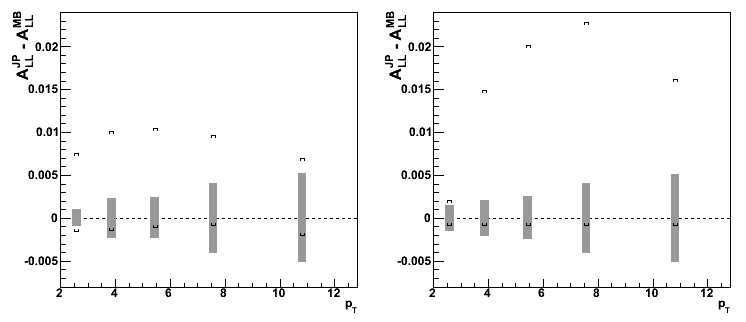
\includegraphics[width=\textwidth]{figures/syst_mcasym_2005}
    \caption{Asymmetry differences used to compute the trigger bias systematic for the 2005 analysis. The square braces represent the maximum asymmetry difference between ``true'' and ``trigger+reco'' Monte Carlo samples assuming a variety of polarized gluon distributions with $\Delta G < 0.3$.  The gray bars represent the maximum statistical uncertainty on the asymmetry difference in each bin.}
    \label{fig:mcasym-2005}
\end{figure}

\begin{table}[ht]
    \begin{center}
        \begin{tabular}{c|c|c}
        \hline
        $p_{T}$ & $\pi^{-}$ $\delta A_{LL}$ & $\pi^{+}$ $\delta A_{LL}$\\
        \hline
        2.00 - 3.18  & -0.0076 +0.0015 & -0.0021 +0.0015\\
        3.18 - 4.56  & -0.0101 +0.0023 & -0.0149 +0.0021\\
        4.56 - 6.32  & -0.0105 +0.0024 & -0.0202 +0.0025\\
        6.32 - 8.80  & -0.0097 +0.0041 & -0.0228 +0.0041\\
        8.80 - 12.84 & -0.0070 +0.0052 & -0.0162 +0.0051\\
    \hline
    \end{tabular}
    \end{center}
    \caption{2005 Trigger and Reconstruction Bias Uncertainties}
    \label{tbl:trig-reco-bias}
\end{table}

\subsubsection{2006 Bias Calculations}

An additional complication for the 2006 data analysis is shown in
Figure~\ref{fig:mean-pt-simu}. The JP trigger efficiency is a sharply-rising
function of jet \(p_T\); as a result, the \(\langle p_T \rangle\) for pions and
especially for jets in a given \(z\) bin is significantly larger in the
triggered sample compared to the minimum-bias sample. In effect, we are
under-sampling the low \(x\) regime in each \(z\) bin. The bias calculated by a
na\"ive application of the Method of Asymmetry Weights to this measurement would
be unacceptably large. Instead, we choose to publish the trigger efficiency as
part of the measurement, and to rescale the minimum-bias Monte Carlo sample by
that trigger efficiency. A comparison of the simulated \(A_{LL}\) in the
triggered and rescaled minimum-bias samples allows an estimate of the
measurement error introduced by the trigger's subprocess bias.

\begin{figure}
  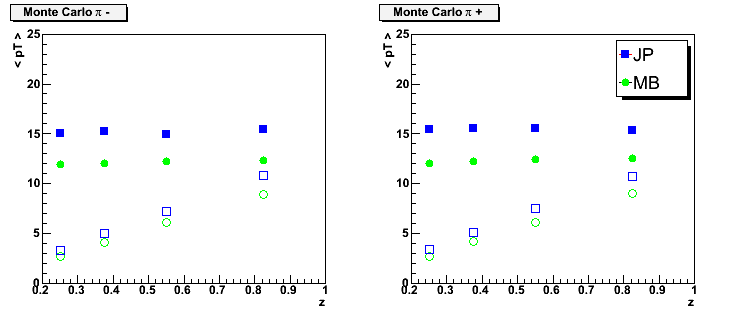
\includegraphics[width=1.0\textwidth]{figures/meanpt-by-trigger}
  \caption{Comparison of the $\langle p_T \rangle$ for MB and JP triggers ni the 2006 Monte Carlo.  Filled markers plot jet $\langle p_T \rangle$ and open markers charged pion $\langle p_T \rangle$. The JP triggered data sample has a dramatically larger jet $\langle p_T \rangle$ in each $z$ bin, which biases $A_{LL}$ towards larger values in the GRSV framework.}
  \label{fig:mean-pt-simu}
\end{figure}

Figure~\ref{fig:trigger-efficiency} plots the ratio of jet yields in the MB
Monte Carlo sample and the sample that passes a simulated JP trigger. The
trigger efficiency as a function of jet \(p_T\) is well described by a cubic
polynomial:
%
\begin{equation}
  \epsilon_{trigger} = 1.149 - 0.2655 * p_T   + 0.01857 * p_T^2 - 0.0003445 * p_T^3.
  \label{eqn:trigger-efficiency}
\end{equation}
%
Finally, Figure~\ref{fig:trig-bias-2006} plots the difference between the
trigger sample \(A_{LL}\) and the \(A_{LL}\) calculated from the rescaled MB
sample for an envelope of GRSV parameterizations with integral gluon
polarization less than 0.3 at \(Q^2 = 1 GeV^2\). A systematic uncertainty on our
measured \(A_{LL}\) is assigned by taking the maximum asymmetry difference in
each bin, or the uncertainty on the triggered \(A_{LL}\) if all asymmetry
differences are consistent with zero. The final values are tabulated in
Table~\ref{tab:trig-bias-2006}.

% TODO reweight 2006 Monte Carlo by DSS/Kretzer ratio

\begin{figure}
  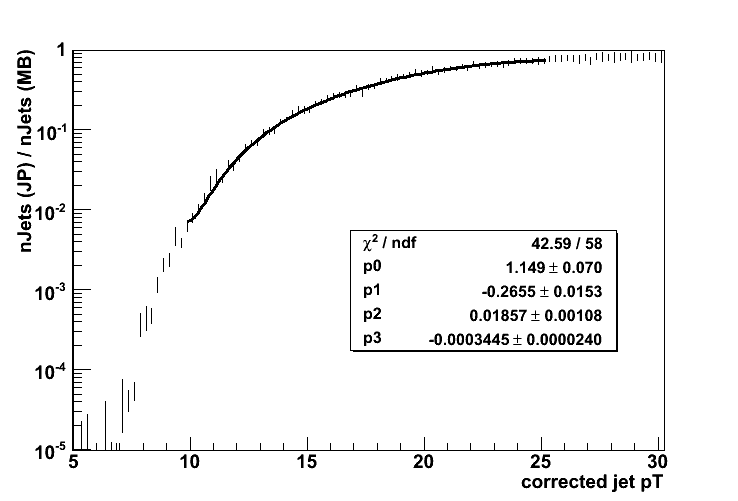
\includegraphics[width=1.0\textwidth]{figures/trigger-efficiency}
  \caption{A parameterization of the BJP1 trigger efficiency as a function of corrected jet $p_T$ established from the 2006 Monte Carlo.  This parameterization is used to factor out the trigger efficiency from the Method of Asymmetry Weights $A_{LL}$ studies, allowing those studies to focus on the subprocess bias inherent in the trigger.}
  \label{fig:trigger-efficiency}
\end{figure}

\begin{figure}
    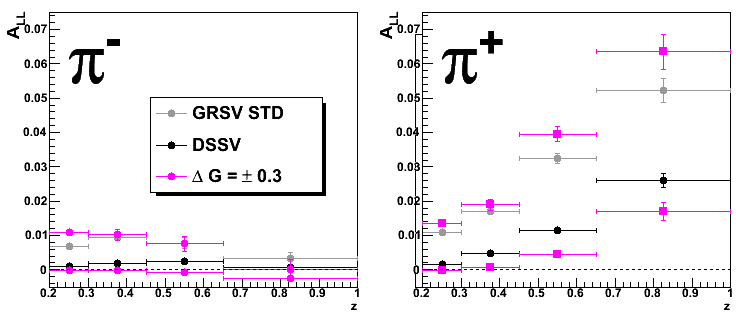
\includegraphics[width=1.0\textwidth]{figures/mb_mcasym_2006}
    \caption{Reweighted Monte Carlo asymmetries for the minimum-bias trigger.  The asymmetries defining the $\Delta G < 0.3$ envelope are used to calculate the systematic uncertainty.  Shown for comparison are the Monte Carlo asymmetries computed assuming two common polarized gluon distributions.}
    \label{fig:mb-mcasym-2006}
\end{figure}

\begin{figure}
  \centering
  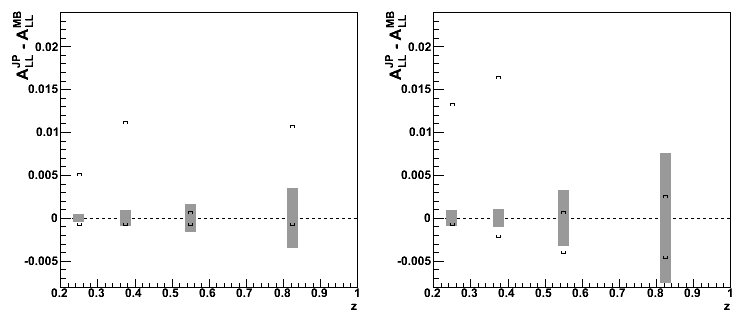
\includegraphics[width=\textwidth]{figures/syst_mcasym_2006}
  \caption{Asymmetry differences used to compute the trigger bias systematic for the 2005 analysis. The square braces represent the maximum asymmetry difference between the rescaled minimum-bas sample and ``trigger+reco'' Monte Carlo samples assuming a variety of polarized gluon distributions with $\Delta G < 0.3$.  The gray bars represent the maximum statistical uncertainty on the asymmetry difference in each bin.  The resulting envelope is a measure of the bias introduced by the subprocess-dependence in the trigger in the 2006 RHIC dataset.}
  \label{fig:trig-bias-2006}
\end{figure}

\begin{table}[ht]
    \begin{center}
        \begin{tabular}{c|c|c}
        \hline
        $z$ & $\pi^{-}$ $\delta A_{LL}$ & $\pi^{+}$ $\delta A_{LL}$\\
        \hline
        0.20 - 0.30  & -0.0052 +0.0005 & -0.0134 +0.0009 \\
        0.30 - 0.45  & -0.0113 +0.0010 & -0.0165 +0.0023 \\
        0.45 - 0.65  & -0.0017 +0.0017 & -0.0032 +0.0040 \\
        0.65 - 1.00  & -0.0108 +0.0035 & -0.0076 +0.0076 \\
    \hline
    \end{tabular}
    \end{center}
    \caption{2006 Trigger and Reconstruction Bias Uncertainties}
    \label{tab:trig-bias-2006}
\end{table}
